\documentclass{article}
\usepackage[polish]{babel}
\usepackage[T1]{fontenc}
\usepackage{amsmath}
\usepackage{gensymb}
\usepackage{float}
\usepackage{graphicx} % Required for inserting images
\graphicspath{ {./images/} }

\title{Laboratorium 10 \\ Równania różniczkowe zwyczajne - część II}
\author{Maciej Borowiec}
\date{04.06.2025}

\begin{document}

\maketitle

\section{Wprowadzenie}
Celem ćwiczenia było zrobienie zadania polegającego na rozwiązaniu układu dwóch równań różniczkowych opisanych modelem Lotki-Volterry różnymi metodami i porównanie tych metod.

\section{Zadanie}
Do opisania układu drapieżca-ofiary możemy użyć modelu Lotki-Volterry:
\begin{equation}
    \begin{cases}
        x' = x(\alpha_1 - \beta_1y) \\
        y' = y(-\alpha_2 + \beta_2x)
    \end{cases} \nonumber
\end{equation}
gdzie:
\begin{itemize}
\item $x(t)$ to gęstość ofiar (np. liczba zajęcy na jednostkę powierzchni) od czasu
\item $y(t)$ to gęstość drapieżców (np. liczba rysi na jednostkę powierzchni) od czasu
\item $\alpha_1$ to współczynnik przyrostu ofiar w izolowanym środowisku
\item $\alpha_2$ to współczynnik ubywania drapieżców w izolowanym środowisku
\item $\beta_1$ to współczynnik intensywności kontaktów między drapieżcami a ofiarami, kończących się upolowaniem ofiary
\item $\beta_2$ to współczynnik opisujący wpływ obecności ofiar na współczynnik przyrostu drapieżców
\end{itemize}
Zadanie należało rozwiązać jawną metodą Eulera, niejawną metodą Eulera, półjawną metodą Eulera oraz metodą Rungego-Kutty czwartego rzędu dla przedziału $[0;80]$. Przyjęto wartości początkowe: $x(0) = 20$, $y(0) = 20$, parametry: $\alpha_1 = 1$, $\beta_1 = 0.1$, $\alpha_2 = 0.5$, $\beta_2 = 0.02$ oraz krok $h = 0.01$.

\subsection{Liczebność populacji w zależności od czasu}
Po rozwiązaniu układu tymi metodami, możemy przedstawić na wykresie otrzymane wyniki. Przedstawimy na początku liczebności populacji w zależności od czasu, a następnie portret fazowy układu.
\begin{figure}[H]
    \centering
    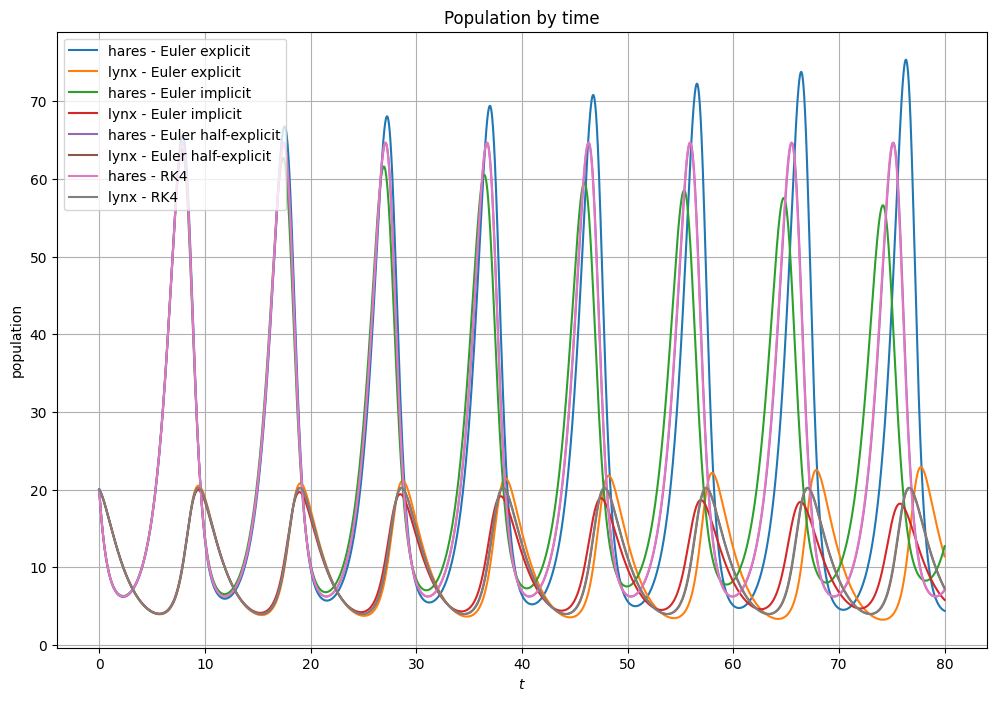
\includegraphics[width=0.95\textwidth]{1}
    \caption{Populacja zajęcy oraz rysi w zależności od czasu dla danych metod}
    \label{fig:mesh}
\end{figure}
Na podanym wykresie (Rysunek 1) widzimy, że dla każdej z metod wynikowe funkcje zachowują się podobnie. Liczba ofiar osiąga wyższe wartości od liczby drapieżców, jednakże przy wzroście rysi liczba zajęcy szybko zaczyna spadać. Wraz z wzrostem czasu różnice w wynikach pomiędzy metodami się powiększają. Natomiast wartości dla metody półjawnej Eulera oraz metody RK4 są tak mało różne, że wykresy na rysunku się pokrywają.
\begin{figure}[H]
    \centering
    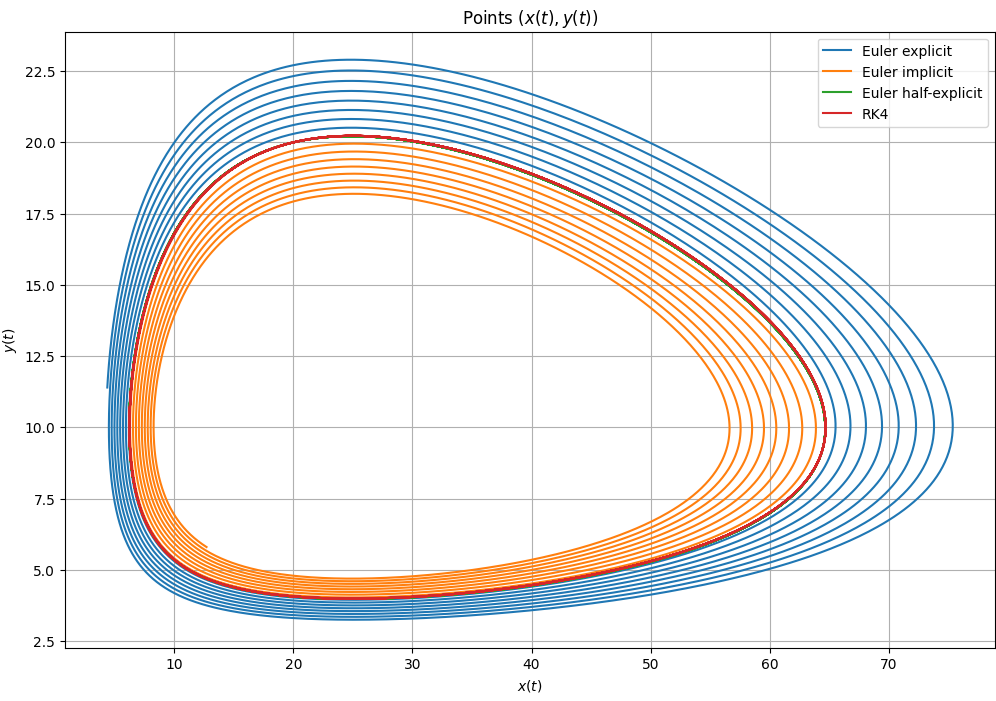
\includegraphics[width=0.95\textwidth]{2}
    \caption{Portret fazowy układu dla danych metod}
    \label{fig:mesh}
\end{figure}
Na danym wykresie (Rysunek 2) łatwo zauważyć formujący się cykl. Można go łatwo wyjaśnić: wraz z wzrostem czasu rośnie populacja zajęcy, wraz z wzrostem populacji zajęcy przybywa więcej rysi, przybycie rysi powoduje zmalenie (poprzez śmierć) populacji zajęcy i wraz z tym maleniem rysie dokonują relokacji.

\subsection{Punkty stacjonarne układu}
Chcemy znaleźć punkty stacjonarne układu, czyli punkty, dla których populacja nie będzie się zmieniać w czasie. Możemy się spodziewać wystąpienia ich (nie wliczając zdegenerowanego przypadku $x=0$, $y=0$) gdzieś w środku danego portretu fazowego widocznego na wykresie wyżej (Rysunek 2). Do znalezienia ich położenia wystarczy rozwiązać układ:
\begin{equation}
    x' = x(\alpha_1 - \beta_1y) = 0
\end{equation}
\begin{equation}
    y' = y(-\alpha_2 + \beta_2x) = 0
\end{equation}
Równanie (1) posiada dwa rozwiązania: $x=0$, $\alpha_1-\beta_1y=0$. Rozpatrzymy zatem dwa przypadki.
\\\\
$1\degree\ x = 0$ - wtedy równanie (2) wygląda następująco:
$$-\alpha_2y = 0$$
Zatem $y$ musi być równy $0$.
\\\\
$2\degree\ \alpha_1-\beta_1y=0 \implies y = \frac{\alpha_1}{\beta_1}$ - wtedy równanie (2):
$$\frac{\alpha_1}{\beta_1}(-\alpha_2 + \beta_2x) = 0$$
To równanie jest spełnione wtw., gdy:
$$-\alpha_2 + \beta_2x = 0$$
Zatem $x = \frac{\alpha_2}{\beta_2}$.
\\\\
Otrzymujemy zatem dwa rozwiązania:
\begin{equation}
    \begin{cases}
        x = 0 \\
        y = 0
    \end{cases} \nonumber
    \begin{cases}
        x = \frac{\alpha_2}{\beta_2} \\
        y = \frac{\alpha_1}{\beta_1}
    \end{cases} \nonumber
\end{equation}
Podstawiając przyjęte wartości parametrów:
\begin{equation}
    \begin{cases}
        x = 0 \\
        y = 0
    \end{cases} \nonumber
    \begin{cases}
        x = \frac{0.5}{0.02} = 25 \\
        y = \frac{1}{0.1} = 10
    \end{cases} \nonumber
\end{equation}
Możemy te punkty przedstawić na wykresie razem z portretem fazowym.
\begin{figure}[H]
    \centering
    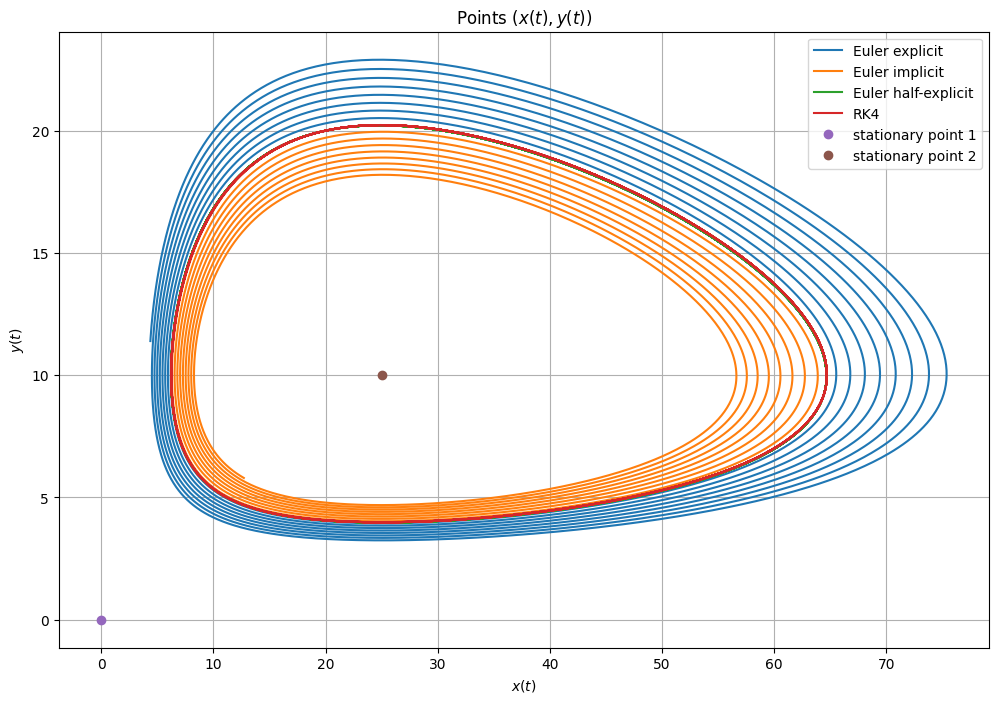
\includegraphics[width=0.95\textwidth]{3}
    \caption{Portret fazowy układu dla danych metod wraz z punktami stacjonarnymi}
    \label{fig:mesh}
\end{figure}
Jak widać na wykresie (Rysunek 3), zgodnie z przewidywaniami, niezdegenerowany punkt stacjonarny znajduje się w "środku" cyklu portretu fazowego.

\subsection{Niezmiennik}
Chcemy zobaczyć, czy dla otrzymanych wyników zachowany jest niezmiennik:
$$H(x,y) = \beta_2x + \beta_1y - \alpha_2\ln x - \alpha_1\ln y$$
W tym celu przedstawimy wykres wartości tego niezmiennika w zależności od czasu dla każdej z metod.
\begin{figure}[H]
    \centering
    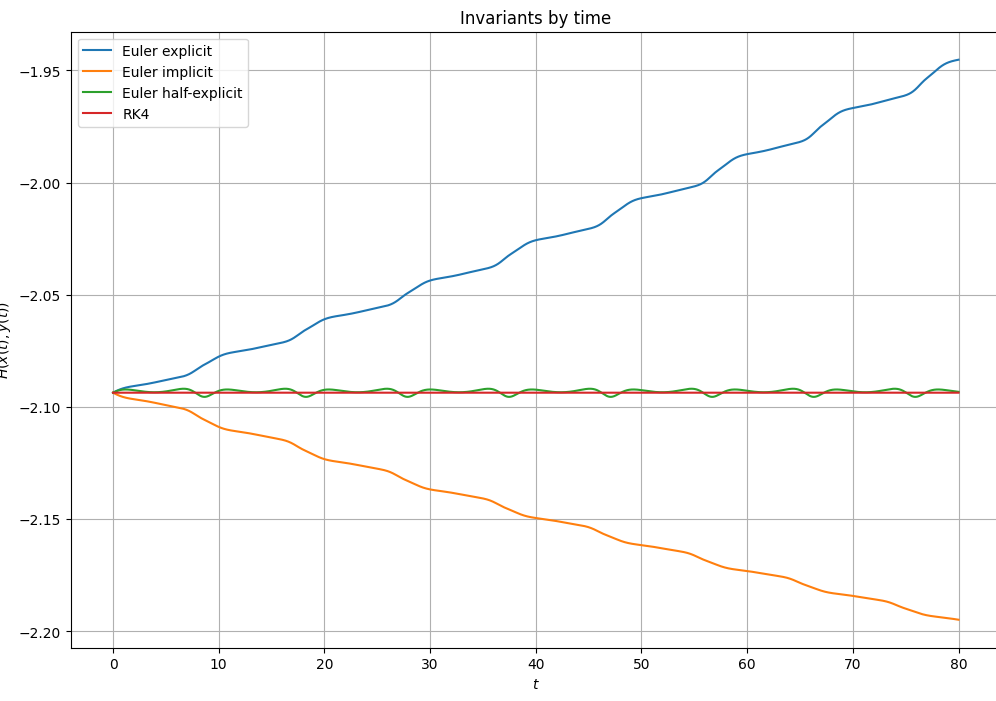
\includegraphics[width=0.95\textwidth]{4}
    \caption{Niezmiennik w zależności od czasu dla danych metod}
    \label{fig:mesh}
\end{figure}
Jak widać na przedstawionym rysunku (Rysunek 4), niezmiennik nie jest zachowany dla metody Eulera jawnej - wzrasta w czasie i metody Eulera niejawnej - maleje w czasie. Może to być zależne od błędu i/lub stabilności tych metod. Dla metody Eulera półjawnej niezmiennik również posiada zmiany w czasie, jednakże są one niewielkie i są ciągle mniejsze od danej stałej, tj. nie wzrasta, ani nie maleje, a oscyluje w okół jednej wartości. Natomiast dla metody Rungego-Kutty czwartego rzędu niezmiennik zachowuje jedną stałą wartość lub zmiany są tak niewielkie, że nie widać ich na wykresie.

\subsection{Znajdowanie parametrów układu dla prawdziwych danych}
Mamy przedstawione prawdziwe dane dla populacji rysi i zajęcy przedstawione w pliku \textbf{LynxHare.txt}. Należało wybrać jedną z danych metod i oszacować prawdziwe wartości współczynników $\alpha_1, \alpha_2, \beta_1, \beta_2$. W tym celu trzeba było dokonać minimalizacji obu z danych niżej funkcji kosztu:
$$L_1(\theta) = \sum_{i=0}((l_i-\hat{l}_i)^2 + (h_i-\hat{h}_i)^2)$$
$$L_2(\theta) = \sum_{i=0}(-l_i\ln\hat{l}_i - h_i\ln\hat{h}_i + \hat{l}_i + \hat{h}_i)$$
gdzie:
\begin{itemize}
\item $l_i$ to prawdziwa liczba rysi w danym roku
\item $\hat{l}_i$ to liczba rysi w danym roku wyliczona metodą numeryczną
\item $h_i$ to prawdziwa liczba zajęcy w danym roku
\item $\hat{h}_i$ to liczba zajęcy w danym roku wyliczona metodą numeryczną
\end{itemize}
Do rozwiązania należało wykorzystać metodę Neldera-Meada, która nie wymaga informacji o gradiencie $\nabla_{\theta}L(\theta)$, którego nie posiadamy.
\\\\
Wykorzystałem metodę półjawną Eulera, gdyż okazała się ona niewiele gorsza w tym przypadku od metody RK4, a jest znacząco mniej intensywna obliczeniowo, gdyż da się ją przedstawić za pomocą jawnego wzoru przedstawionego poniżej:
\begin{equation}
    \begin{cases}
        y_{n+1} = \frac{y_n}{1 - h(-\alpha_2+\beta_2x_n)} \\
        x_{n+1} = x_n + hx_n(\alpha_1-\beta_1y_{n+1})
    \end{cases} \nonumber
\end{equation}
Poniżej przedstawiona została tabela z wynikami minimalizacji.
\begin{table}[h!]
    \centering
    \begin{tabular}{|c|c|c|c|c|c|}
        \hline
        & $\alpha_1$ & $\alpha_2$ & $\beta_1$ & $\beta_2$ & Koszt \\
        \hline
        Parametry początkowe & $1$ & $0.5$ & $0.1$ & $0.02$ & - \\
        1. funkcja kosztu & $1.6721$ & $0.1831$ & $0.0612$ & $0.0043$ & $115128.9315$ \\
        2. funkcja kosztu & $1.0266$ & $0.3850$ & $0.0443$ & $0.0108$ & $-17575.2789$ \\
        \hline
    \end{tabular}
    \caption{Wyniki minimalizacji obu funkcji kosztu}
    \label{table}
\end{table}
\\
Rozwiązania widoczne w tabeli wyżej (Tabela 1) są różne dla obu funkcji kosztu. Może to oznaczać niedokładność metody półjawnej Eulera lub niedokładność metody optymalizacji Neldera-Meada. Może to również oznaczać, że istnieje wiele kombinacji parametrów, które wystarczająco dokładnie opisują nasze dane, przez co znalezione zostały dwa różne lokalne minima.

\section{Podsumowanie}
Dane zadanie pokazało zastosowanie zagadnienia rozwiązywania układów równań różniczkowych w praktyce. Dzięki prawdziwym danym populacji rysiów i zajęcy mogliśmy otrzymać układ opisujący dane środowisko i przewidzieć zmiany w populacji w przyszłości. To zadanie pokazało również dwie nowe (w stosunku do poprzedniego laboratorium) metody rozwiązywania układów równań różniczkowych. Metoda Eulera półjawna i metoda Rungego-Kutty czwartego rzędu okazały się w tym zadaniu dużo lepsze. Metoda RK4 była najdokładniejsza, lecz metoda półjawna Eulera również była bardzo dokładna. Do tego, posiadała ona prosty wzór, dzięki czemu optymalizacja używając tej metody była znacznie mniej wymagająca obliczeniowo i, co za tym idzie, dużo szybsza od optymalizacji przy użyciu metody RK4.

\section{Bibliografia}
\begin{itemize}
\item Materiały zamieszczone wraz z zadaniem
\end{itemize}

\end{document}
